
%(BEGIN_QUESTION)
% Copyright 2015, Tony R. Kuphaldt, released under the Creative Commons Attribution License (v 1.0)
% This means you may do almost anything with this work of mine, so long as you give me proper credit

\noindent
{\bf RTU component layout}

\vskip 10pt

An ``RTU'' is a {\it Remote Terminal Unit} in a SCADA system serving as the interface between field instruments and a central control/display unit called the ``MTU'' ({\it Master Terminal Unit}).  In our caSCADA system, the MTU is just a laptop computer viewing data generated by the Raspberry Pi computer in each RTU.  Each RTU uses a LabJack data acquisition unit to sense analog signals sent by field transmitters and a single-board computer called a Raspberry Pi to condition and present that data in the form of digital data files readable by the MTU.  Communication takes place via a wireless access point (WAP) router:

$$\includegraphics[width=15.5cm]{i02566x01.eps}$$

Each RTU enclosure is weatherproof, and equipped with a set of batteries to maintain DC power to all the system components in the event of an external AC power failure.

The upper level of terminals on the triple-level blocks should all be jumpered together because this is the 20 VDC ``bus'' used to power all field instruments.  The lower level of terminals should also be jumpered together because they comprise the negative side (``Common'' or ``GND'') of that same 20 VDC loop power supply.





\vfil \eject

\noindent
{\bf Sample loop diagrams}

$$\includegraphics[width=15.5cm]{i02566x02.eps}$$

A set of triple-height terminal blocks marshall field instrument signals to the DAQ input terminals.  Both current-based and voltage-based instrument signals may be accepted by the DAQ.  In the case of 4-20 mA loop instruments, a precision 250 $\Omega$ resistor is connected in such a way to provide a 1-5 VDC signal for the DAQ to sense.  If the field instrument outputs a voltage signal instead (which is actually quite common for RTU loops in remote installations relying on solar power) then the resistor is omitted and the LabJack AIN directly reads that instrument's output voltage.

\vskip 10pt

All $n$ terminals are jumpered together and powered by the same 20 VDC source, fed through fuse \#1.  All $4n$ terminals are also jumpered together and connect to the negative rail of the 20 VDC power source.  Only the $2n$ terminals are independent from each other, since they carry the individual analog input signals unique to each AIN channel on the LabJack.



\vfil \eject

\noindent
{\bf Electrical power diagram}

$$\includegraphics[width=15.5cm]{i02566x03.eps}$$

Power is sent to each RTU box at 12 volts AC, from a transformer located near a 120 VAC power source.  This keeps the field power cable at a safe, low voltage (similar to outside sprinkler control systems and walkway lighting). 

\vskip 10pt

Internal to each RTU is a dual-voltage DC system: 12 volts (regulated down to 5 VDC) for running the Linux-based computer, LabJack DAQ, and Linksys WRT54GL wireless router; and 20 volts for powering the field instruments.  Lead-acid batteries provide back-up power for the RTU to continue running in the event of a power outage.  The resistor-diode network limits battery charging current to a bare minimum, while providing full current capacity in the discharge direction (in the event of an AC line power outage).

24 volts is a more customary DC supply voltage for loop-powered field instruments, but the LabJack model T7 DAQ has an absolute maximum input voltage of 20 VDC.  Thus, the loop supply voltage is limited to this value to avoid the potential for damage to the LabJack in the event of a shorted instrument cable which would apply full power supply voltage to the DAQ input.





\vfil \eject

\noindent
{\bf RTU power system testing procedure}

\vskip 10pt

You must follow this procedure when first commissioning a new RTU.  When working with an existing RTU, you may follow the same procedure to test the continuing health of the DC power system.

\vskip 10pt

\begin{itemize}
\item{(1)} Test the external 12 VAC transformer by itself: when plugged into a 120 volt AC source, does it output at least 12 volts AC?
\vskip 10pt
\item{(2)} Open up all fuses (\#1 through \#5) to ensure no device will become powered until you intend so.
\vskip 10pt
\item{(3)} Connect this external 12 VAC transformer's output to the RTU as shown in the diagrams and apply power.  Check the output of both bridge rectifiers for proper DC voltage magnitude and polarity.  Due to the filter capacitors the DC voltage magnitudes will register greater than the AC voltage magnitudes feeding each of the bridge rectifiers.
\vskip 10pt
\item{(4)} Ensure the batteries are wired to the proper terminal blocks and fuse holders, and measure DC voltage magnitudes and polarities at the battery-side of each open fuse.  This ensures the batteries are properly connected.
\vskip 10pt
\item{(5)} Close fuses \#2 and \#4.  This connects the two battery banks to their respective charging sources.  Re-measure the voltage magnitudes at the battery-side of each closed fuse.  You should read slightly higher voltage now than in the previous step, because the batteries are charging.
\vskip 10pt
\item{(6)} Ensure all power plugs are removed from the caSCADA electronic devices: the LabJack DAQ unit, the Raspberry Pi computer, and the Linksys wireless router.  Prepare to measure DC voltage at the ends of those power plugs.
\vskip 10pt
\item{(7)} Close fuse \#3 and measure DC voltage magnitude and polarity at the Linksys router's power plug.  Check the router's documentation for the proper DC polarity of the plug's shell and tip to see that the polarity is correct.  If all is well, plug the power cable into the router and check to see that it powers up.  Re-measure voltage magnitude at fuse \#3 to see that the router is receiving adequate voltage while powered (i.e. under load).
\vskip 10pt
\item{(8)} Close fuse \#5 and measure DC voltage magnitude and polarity at the Raspberry Pi's micro-USB power plug.  Check online for the ``pinout'' specification of a micro-USB power plug to see that the polarity is correct.  If the pins on the micro-USB plug are too small to safely probe using your multimeter, you may check DC voltage at the stripped end of that cable where it lands at the terminal block, and verify correct voltage and polarity according to the colors of that cable's wires.  If all is well, plug the power cable into the Raspberry Pi and check to see that it powers up.
\vskip 10pt
\item{(9)} Plug the B-style USB cable into the LabJack.  It receives power through the Raspberry Pi and should power up immediately.  Re-measure voltage magnitude at fuse \#5 to see that both the Raspberry Pi and LabJack units are receiving adequate voltage while powered (i.e. under load).
\vskip 10pt
\item{(10)} Close fuse \#1 to apply 20 VDC power to the field instrument terminal blocks.  Measure DC voltage magnitude and polarity between terminals 13 and 53 to ensure 20 VDC is supplied all the way to the end of the terminal block section.
\vskip 10pt
\item{(11)} At this point in time you may initialize the caSCADA system MTU (a laptop PC) and test the system for proper data.  A procedure for this is given on the following page.
\vskip 10pt
\item{(12)} Unplug the external 12 VAC transformer from its line power source, and re-measure all DC supply voltages to ensure all devices are receiving adequate voltage under battery power alone.
\vskip 10pt
\item{(13)} Repeat these DC voltage measurements at one-hour intervals to check the health of the batteries.
\end{itemize}





\vfil \eject

\noindent
{\bf RTU data system testing}

\vskip 10pt

You must follow this procedure when first commissioning new devices for an RTU.

\vskip 10pt

\begin{itemize}
\item{(1)} Ensure that the proper IP addresses are all written on labels affixed to each of the networked devices in the RTU: the LabJack DAQ unit, the Linksys wireless router, and the Raspberry Pi single-board computer.
\vskip 10pt
\item{(2)} Set the IP address and subnet mask of your personal computer to appropriate values for the Ethernet device you wish to connect to.  For each octet of the subnet mask with the value ``255'' the octet of your PC's IP address must match the IP addresses of all devices in the RTU.  For each octet of the subnet mask with the value of ``0'' the octet of your PC's IP address must be different from any device in the RTU.  This will prepare your PC for direct Ethernet cable connection to the device you intend to configure.  
\vskip 10pt
\item{(3)} Plug your computer into the Linksys router using an Ethernet cable, and set the router's IP address and subnet mask and name using a web browser.  Follow the instructions given in the manual for the router.  The router's name should make sense to any user of the system.  In an area with multiple RTUs, the name should be specific enough to clearly identify which RTU it is.
\vskip 10pt
\item{(4)} Plug your computer into the LabJack DAQ using an Ethernet cable, and set the DAQ's IP address and subnet mask using the software provided by LabJack for this task.  Follow the instructions given in the LabJack manual.
\vskip 10pt
\item{(5)} Plug an HDMI monitor and USB keyboard into the Raspberry Pi, and log in directly to set its IP address and subnet mask.  To check its current settings, use the {\tt ifconfig} command (similar to the {\tt ipconfig} command in Microsoft Windows).  If the settings are not correct, you may change them by editing the file {\tt /etc/network/interfaces}.  This requires ``root'' privileges.  Lines of text in this {\tt interfaces} file follow this pattern:
\begin{itemize}

\item{} Prior to the {\tt eth0} line must be a line that reads {\tt auto eth0}
\item{} The ``address'' line contains the IP address (e.g. {\tt address 169.254.8.3})
\item{} The ``netmask'' line contains the subnet mask (e.g. {\tt netmask 255.255.255.0})
\vskip 10pt
\item{(6)} Unplug the Ethernet cable from your personal computer and wirelessly connect to the Linksys router.  The router will automatically assign an appropriate IP address to your computer's wireless card, as routers are designed to do.
\vskip 10pt
\item{(7)} Use the {\tt ping} command in your computer to test network connectivity with each device in the RTU.  This command is simply the word ``ping'' followed by the IP address of the device you wish to ping.  For example, {\tt ping 169.254.8.1} will test to see whether your computer has connectivity with the device bearing the IP address 169.254.8.1.
\vskip 10pt
\item{(8)} Once all devices have been proven to ping successfully, you may use an SSH client program in your personal computer (e.g. {\tt Bitvise}) to log into the Raspberry Pi.  The login account is simply {\tt btc} with the password {\tt btc}.
\vskip 10pt
\item{(9)} Once you are logged in to the Linux operating system in the Raspberry Pi, you may try compiling the caSCADA code and then running it (either the {\tt simulate} process or the {\tt poll} process) to see that the data files are being appropriately populated by the caSCADA software.
\end{itemize}






\vfil \eject

\noindent
{\bf Preparing the Raspberry Pi for use in the caSCADA system}

\vskip 10pt

If you are initially configuring a Raspberry Pi to be used in the caSCADA system, there are several things you must do.  This is outside the realm of student work, and will be completed by the instructor prior to your use of the Raspberry Pi.  Here is a list:

\begin{itemize}
\item{} Log in as the default user (name = {\tt pi} and password = {\tt raspberry})
\vskip 5pt
\item{} Use the {\tt sudo} and {\tt passwd} commands to reset the root account's password to your liking (e.g. {\tt sudo passwd root}).  There are several tasks for which root privileges are necessary, so it's convenient to be able to log into the root account and do that work there, rather than have to preface all those commands typed under the {\tt pi} login user with the ``{\tt sudo}'' qualifier.
\vskip 5pt
\item{} Use the {\tt raspi-config} utility to set the system's hostname, configure the keyboard for US mapping (as British ``UK'' mapping is the default!), and also enable the {\tt ssh} server which will be essential for remote login and system administration.
\vskip 5pt
\item{} Add a new user account called {\tt btc}.
\vskip 5pt
\item{} Feel free to edit the hidden file named {\tt .profile} in the {\tt /home/btc} directory with any special instructions to be executed at login.  For example, you may add lines containing the {\tt echo} shell command to print messages to the screen for the user once they log in (e.g. {\tt echo "Welcome to the fish hatchery RTU"}). 
\vskip 5pt
\item{} Set the current time and date using the {\tt date} command.  The format is MMDDhhmmCCYY.  For example, 3:21 PM on November 5, 2016 would be set by issuing the command {\tt date 110515212016}.
\vskip 5pt
\item{} Navigate to the {\tt /etc/network} directory and edit the file named {\tt interfaces} to set all the required IP address and netmask information to give the Raspberry Pi a static IP address for use in the caSCADA system.
\vskip 5pt
\item{} Install the {\tt cascada.tar} archive file in the {\tt /home/btc} directory, and then use the command {\tt tar xvf cascada.tar} to unpack that archive file.
\vskip 5pt
\item{} Install the latest {\tt libmodbus} library archive file in the {\tt root} directory, then uncompress it ({\tt gunzip libmodbus*.gz}) and unpack the archive ({\tt tar xvf libmodbus*tar}) and then descend into the new {\tt libmodbus} directory to build it.  Build and install the new software using the commands {\tt ./configure ; make ; make install ; ldconfig}.
\vskip 5pt
\item{} Install the latest {\tt ncurses} library archive file in the {\tt root} directory, then uncompress it ({\tt gunzip ncurses*.gz}) and unpack the archive ({\tt tar xvf ncurses*tar}) and then descend into the new {\tt ncurses} directory to build it.  Build and install the new software using the commands {\tt ./configure ; make ; make install ; ldconfig}.
\vskip 5pt
\item{} Install the latest {\tt lynx} text-based web browser software archive file in the {\tt root} directory, then uncompress it ({\tt gunzip lynx*.gz}) and unpack the archive ({\tt tar xvf lynx*tar}) and then descend into the new {\tt lynx} directory to build it.  Build and install the new software using the commands {\tt ./configure ; make ; make install ; ldconfig}.
\vskip 5pt
\item{} Navigate to the {\tt /home/btc} directory and edit the file {\tt cascada\_poll.c} with the correct IP address to establish a Modbus/TCP connection with the LabJack DAQ unit in your RTU.  The function establishing the address will be easy to find in this file, as it calls out the IP address in standard four-octet format.  Just edit the IP address that's shown, and the caSCADA software will be able to communicate with that LabJack DAQ.
\vskip 5pt
\item{} Try running {\tt make poll} and {\tt make simulate} in the {\tt /home/btc} directory to see that the caSCADA software successfully compiles.
\end{itemize}




\underbar{file i02566}
%(END_QUESTION)





%(BEGIN_ANSWER)


%(END_ANSWER)





%(BEGIN_NOTES)


%INDEX% Lab exercise, diagrams for caSCADA system RTUs

%(END_NOTES)


